\documentclass[conference, twoside]{IEEEtran}
\IEEEoverridecommandlockouts
% The preceding line is only needed to identify funding in the first footnote. If that is unneeded, please comment it out.
\usepackage{cite}
\usepackage{amsmath,amssymb,amsfonts}
\usepackage{algorithmic}
\usepackage{graphicx}
\usepackage{textcomp}
\usepackage{xcolor}
\usepackage{stfloats}
\usepackage{multirow}
\usepackage{listings}
\usepackage{lipsum}
\usepackage{import}
% listing settings
\lstset{
  frame = lines,
  language = C,
  basicstyle = \ttfamily\footnotesize,
  breaklines = true,
}
% listing caption redefinition
\makeatletter
\def\lst@makecaption{%
  \def\@captype{table}%
  \@makecaption
}
\makeatother

\def\BibTeX{{\rm B\kern-.05em{\sc i\kern-.025em b}\kern-.08em
    T\kern-.1667em\lower.7ex\hbox{E}\kern-.125emX}}

\begin{document}

\bstctlcite{IEEEexample:BSTcontrol} % remove dashed repeated authors

\title{Investigating Performance Improvements\\in Discrete Space Hartree-Fock Calculations\\Through Graphics Processing Units\\{\large EECE542 Final Project Report}}
\author{\IEEEauthorblockN{Michel Kakulphimp}
\IEEEauthorblockA{\textit{Dept. of Electrical and Computer Engineering}\\
\textit{University of British Columbia}\\
Vancouver, Canada\\
michel@kakulphimp.net}
}

\markboth{UBC Winter 2021 EECE542: Nanoscale Modelling and Simulations}%
{}
\maketitle

\section{Introduction} % Complete

Graphics processing units (GPUs) have been a mainstay of the computing world for many decades now, thanks in large part to an ever-evolving need to push more and more pixels to displays to showcase a rich variety of real-time graphics and media. At their core, however, they are programmable devices used to perform application-specific computations. It is unsurprising then that GPUs can be leveraged to process other types of workloads. This report outlines a short investigation on how GPUs can be leveraged to accelerate molecular simulation algorithms, specifically the Hartree-Fock method.

\section{Background} % Complete

The following sections provide a brief overview of the Hartree-Fock method as well as GPU acceleration. The information provide should provide enough context to understand how the investigation was able to obtain the results presented towards the end of the report.

\subsection{Hartree-Fock Method} % Complete

The Hartree-Fock (HF) method \cite{szabo-ostlund} is designed to help approximate a solution to the Schr\"{o}dinger equation for many-electron systems. This is accomplished by making some key approximations, including: the Born-Oppenheimer approximation to fix the kinematics of the nucleus, using a single Slater determinant composed of orthogonal molecular spin orbitals to satisfy the Pauli exclusion principle, and most importantly approximating the Hamiltonian as a single electron function by treating the other electrons in the system as a mean field rather than evaluating with their exact states. HF iteratively converges to its solution by progressively making better guesses at the structure of the mean field of the system. Combined, these techniques help reduce the original multivariate and computationally intensive problem into one that is easily solved by a computer program. One such implementation is described within this report, where we perform the restricted, closed-shell HF algorithm on a Helium atom.

Since Helium has an even number of electrons that close shells, we can use the restricted HF (RHF) equation for closed shell systems to numerically calculate the resulting orbitals. The equation is as follows:

\begin{align}
  \hat{F}(\vec{r})\psi_n(\vec{r}) &= \epsilon_n\psi_n(\vec{r})
\end{align}

Where $\hat{F}(\vec{r})$ is the Fock operator which is defined as follows:

\begin{align}
  \hat{F}(\vec{r}) &= \hat{H}_{core}(\vec{r}) + \sum_{n=1}^{N/2}\left[2J_n(\vec{r}) - K_n(\vec{r})\right]
\end{align}

The Fock operator is composed of the core Hamiltonian operator $\hat{H}(\vec{r})$, the Coulomb operator $\hat{J}(\vec{r})$, and the exchange operator $\hat{K}(\vec{r})$.

\begin{align}
  \hat{H}_{core}(\vec{r}) &= -\frac{1}{2}\nabla_1^2 - \sum_A\frac{Z_A}{\|\vec{r}_{1 A}\|}\\
  \hat{J}_j(\vec{r}_1)\psi_i(\vec{r}_1) &= \psi_i(\vec{r}_1)\int_{-\infty}^{\infty}\left|\psi_i(\vec{r}_2)\right|^2\frac{1}{\|\vec{r}_{12}\|}d\vec{r}_2 \\
  \hat{K}_j(\vec{r}_1)\psi_i(\vec{r}_1) &= \psi_j(\vec{r}_1)\int_{-\infty}^{\infty}\frac{\psi_j^\ast(\vec{r}_2)\psi_i(\vec{r}_2)}{\|\vec{r}_{12}\|}d\vec{r}_2
\end{align}

By discretizing the solution space of the problem into $N$ partitions in the three Cartesian coordinate directions and representing the Fock equation in matrix form, we can solve for the discretized wave equation $\psi_n(\vec{r})$ by solving for the eigenvectors of the Fock matrix. For each iteration of the HF algorithm, a new guess is obtained for the discretized wave equation, which can be used to compute the Fock matrix for the following iteration. If initial conditions are favorable, the iterations will eventually settle on a solution with little to no variation. The numeric value of the total energy of the system on every iteration can be used as an indicator for convergence.

This report does not take the concept of HF further than what is presented; however, it is important to note that there is are numerous improvement on the technique. One such improvement uses the Roothaan-Hall equations, by representing the solution wave functions through a linear combination of known spatial basis equations. This allows HF to take another matrix form and has the benefit of being much lighter in terms of computation. Since the techniques discussed in the report target fundamental computations shared by HF and its derivatives, they can of course be applied to them as well.

\subsection{GPU Acceleration} % Complete

GPUs are primarily designed to accelerate and support the computational requirements of real-time raster 3D graphics. However, their hardware is also well suited for accelerating other, highly parallelizable workloads, such as molecular simulations \cite{electronic-structure-calculations-on-gpus}. This is made possible through GPU manufacturers providing APIs that allow developers to write specially designed software to run on the GPU processing units. Since GPUs have a fundamentally different architectures than CPUs, the software must be written with the architecture in mind and must also be compiled as a separate executable entity to be run exclusively on the GPU.

In GPU terminology, the host is the CPU that the GPU is coupled to and the device is the GPU itself. The host is what will be running the main program and the device will be executing offloaded accelerated portions of the main program. The device is connected to the host via a peripheral component interconnect, which by modern standards will likely be PCIe. The host and device each have their own pools of memory which are directly inaccessible from one another, referred to as RAM for the host and video RAM (VRAM) for the device. The functions running on the device are called kernels. When a developer is designing a kernel, the API provides mechanisms to define how that kernel will be parallelized on the device. This would allow, for example, the developer to slice up a problem among the GPU's processing units in a programmatic way.

NVIDIA, a GPU manufacturer, provides one such API for developers called Computer Unified Architecture or CUDA. It is also known as the CUDA parallel computing platform \cite{nvidia-cuda}. CUDA is only available for NVIDIA GPU hardware, but there also exists an alternative that works on other GPU vendors called OpenCL. Since an NVIDIA-based GPU was available for use in this project, CUDA was chosen as the API for GPU acceleration.

At its core, a modern GPU is designed to maximize the throughput of a parallel workload. Given the nature of graphics displays and the millions of pixels contained within them, this architecture makes sense. While the exact implementation details will vary depending on the GPU vendor and the capabilities that are designed into them, one can generally expect them to contain clusters of numerous processing units with varying levels of memory found throughout the device. Due to how these clusters are interconnected, there are limitations to how the processors can access memory within the system. This also limits the flexibility of the processors to perform incongruous tasks within the clusters. All of these architectural considerations must taken into account when developing for a given GPU platform.

\subsection{Development and Architectural Considerations} % Complete

In an example implementation of GPU acceleration, a developer identifies workloads that are well suited for the architecture of a GPU to accelerate and write kernels to be executed exclusively on the GPU. The host program would then call these kernels and provide the necessary data for the device to perform execution and return results. There are three major optimizations that take place during this development process: parallel efficiency, memory throughput, and instruction throughput.

Parallel efficiency relates to optimizing the amount of parallel execution that is exploited on the GPU, which exposes as much parallelism as possible in the accelerated kernels. The architecture of the GPU provides the means to invoke a great deal more parallel code execution when compared to a CPU. However, these massively parallel pipelines rely on code that is executing the same type of operation. For example, heavy performance penalties can occur if numerous branching logic exists in the path of a kernel running on a GPU thread as other threads may stall while the block is used incongruously.

Memory throughput must also be optimized as there are different pools of memory to consider. The GPU has some memory that is private per thread, private per certain number of blocks of threads, and memory that is available to all devices in the GPU. There is of course also the main pool of memory that exists in the host system. Moving between host and device incurs the largest penalty as the memory is copied across the interconnect fabric (PCIe). Care must be taken when designing applications to properly place data within these memories to hide as much memory access latency as possible.

Optimizations in instruction throughput relates to ensuring that the GPU execution units are kept busy in order to reduce idle time. This efficiency is impacted by factors such as data residency (local or global) and synchronization requirements between threads. Global memory access would stall execution until data can be moved into local storage and thread synchronization would occur if there is a data dependency between two threads.

\section{Acceleration Opportunities}

In the HF computation, the core Hamiltonian is computed only once, and this data is resident in memory for the iterations to use when solving for the eigenvectors of the solution. Accelerating any portion of this would not yield significant performance increases for the program, especially if the convergence percentage is small enough to result in a long convergence pattern. This largely leaves the numerical integration and the eigensolver up for acceleration opportunities. This section explores these two computations and how they can be accelerated on a GPU.

\subsection{Numerical Integration}

Performing the numerical integration is straightforward on a GPU. This is largely a result of the program only needing to iterate sequentially once over all of the possible coordinates of the solution space. This allows the input data to be cleanly subdivided into smaller chunks of work to be performed in a massively paralleled manner on the GPU.

\subsection{Eigensolver}

Solving for the eigenvalues and eigenvectors requires the implementation of a diagonalization algorithm. Since the Fock matrix is real and symmetric, a divide-and-conquer algorithm can be used. As these algorithms are generally well studied and implemented in common linear algebra routines, re-implementing them from scratch would likely not be worth the effort. As outlined in the following sections, libraries were found for both the CPU and GPU implementations of the eigensolver.

\section{Implementation} % Complete

The following sections discuss the software libraries used in the program, as well as some of the program architectural details to illustrate how the program's different components eventually come together to provide the results.

\subsection{Software Libraries} % Complete

For this investigation, a program written in C++ was created to evaluate the acceleration of the eigensolver and the numerical integration on a discrete space HF solver for the Helium atom. The program is designed to be able to variably define the number of partitions used in the discretization of the solution space and selectively run the eigensolver and numerical integration on either the CPU or the GPU.

As stated previously, the GPU acceleration framework chosen for this investigation is the CUDA Parallel Computing Platform. Consequently, C++ was chosen as the programming language as it is straightforward to integrate with the CUDA C APIs and the language has wide support in terms of libraries for utilities. CUDA provides its own compiler which compiles source files with the \texttt{.cu} suffix into GPU executable code.

To facilitate the linear algebra operations required by HF, the Eigen \cite{eigen} C++ template library was chosen. This provides structures and types to support matrix arithmetic. Eigen was linked with AMD Basic Linear Algebra Subprograms (BLAS) libraries \cite{amd-blas} to provide low level multi-core CPU support for matrix operations. Eigen was also linked with LAPACK (Linear Algebra PACKage) \cite{lapack} libraries which are used in higher-level linear algebra operations such as those to compute the eigenvectors and eigenvalues of a matrix. OpenMP is used to enable multiprocessor support for the CPU BLAS and LAPACK operations, and the LAPACKE C API is used to wrap around the LAPACK libraries which are written in FORTRAN.

On the CPU-side, the LAPACK \texttt{SSYEVD} function is used to compute the eigenvalues and eigenvectors of the Fock matrix. This function provides a single precision floating point divide-and-conquer algorithm for real symmetric matrices, of which the Fock matrix is one. The AMD BLAS routines are designed to utilize all of the available cores of the system, so the CPU implementation of the diagonalization of the Fock matrix is at its peak performance capability. For the GPU side, the CUDA cuSOLVER library is used to implement the GPU linear algebra routines.

Finally, the C++ Boost libraries provide the program with quality of life tools for things such as command line arguments parsing and string formatting.

\begin{figure*}[ht] % approximately here, at the top
\centering
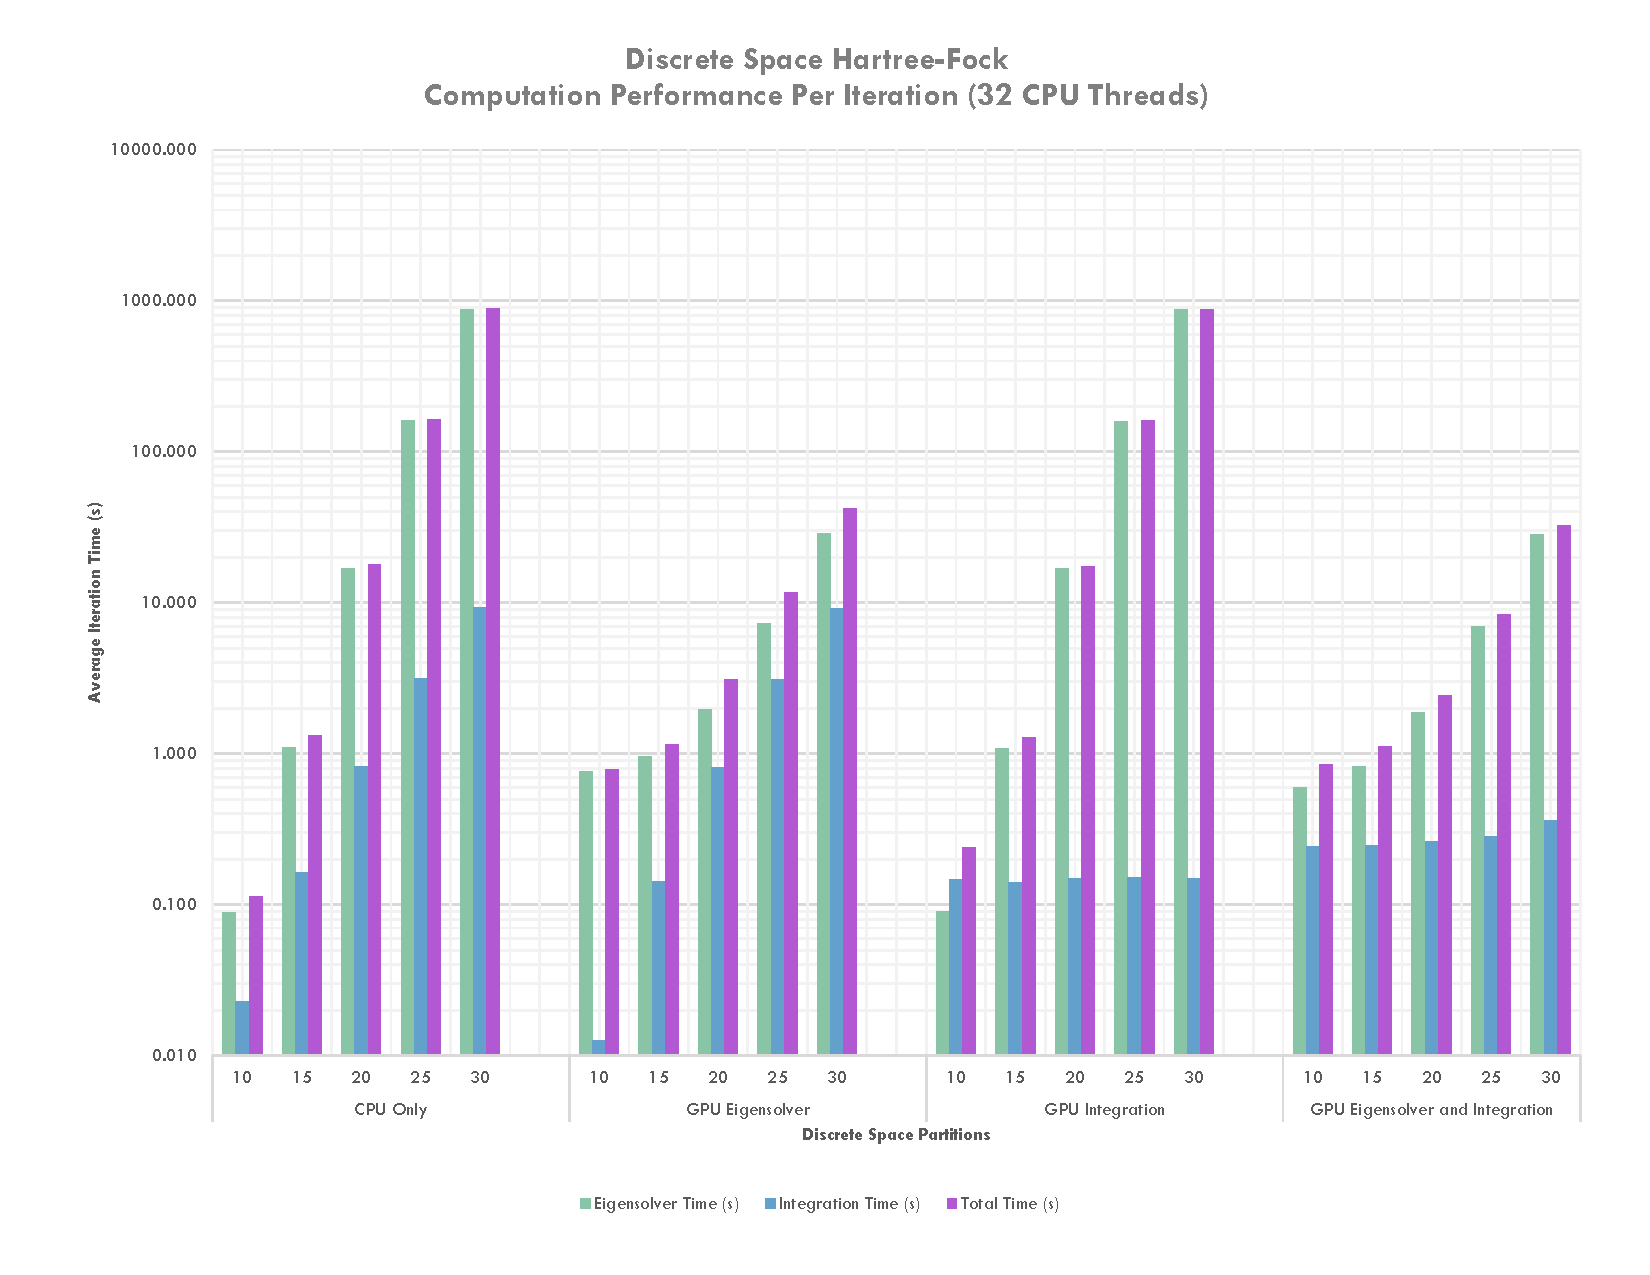
\includegraphics[width=7in]{figures/thirtytwo-thread-results.pdf}
\caption{Performance Results Per Iteration (32 CPU Threads)}
\label{perf-results-per-iteration-thirtytwo-thread}
\end{figure*}

\begin{table*}
    \renewcommand{\arraystretch}{1.3} % vertically stretch table out
    \caption{Computation Performance per Iteration for a Given Mode and Partition Size}
    \label{numeric-results}
    \centering
    \begin{tabular}{|c||c|c|c|c|c|}
        \multicolumn{6}{c}{CPU Only Results} \\
        \hline
        {Solution Partitions} & {10} & {15} & {20} & {25} & {30} \\
        \hline
        \hline
        {Eigensolver Time (s)}              & {0.0884} & {1.0962} & {16.853} & {160.63} & {877.85}\\
        {Integration Time (s)}              & {0.0228} & {0.1649} & {0.8228} & {3.1488} & {9.3617}\\
        {Total Time (s)}                    & {0.1141} & {1.3169} & {17.977} & {164.99} & {891.47}\\
        \hline
    \end{tabular}
    \begin{tabular}{|c||c|c|c|c|c|}
        \multicolumn{6}{c}{GPU Eigensolver Results} \\
        \hline
        {Solution Partitions} & {10} & {15} & {20} & {25} & {30} \\
        \hline
        \hline
        {Eigensolver Time (s)}              & {0.7677} & {0.9546} & {1.972}  & {7.3264} & {28.903}\\
        {Integration Time (s)}              & {0.0125} & {0.1433} & {0.8101} & {3.123}  & {9.1942}\\
        {Total Time (s)}                    & {0.7835} & {1.1514} & {3.0773} & {11.789} & {41.99} \\
        \hline
    \end{tabular}
    \begin{tabular}{|c||c|c|c|c|c|}
        \multicolumn{6}{c}{GPU Integration Results} \\
        \hline
        {Solution Partitions} & {10} & {15} & {20} & {25} & {30} \\
        \hline
        \hline
        {Eigensolver Time (s)}              & {0.0905} & {1.0869} & {16.844} & {159.43} & {880.25}\\
        {Integration Time (s)}              & {0.1473} & {0.1396} & {0.1488} & {0.1514} & {0.1491}\\
        {Total Time (s)}                    & {0.2411} & {1.2816} & {17.295} & {160.71} & {883.72}\\
        \hline
    \end{tabular}
    \begin{tabular}{|c||c|c|c|c|c|}
        \multicolumn{6}{c}{GPU Eigensolver \& GPU Integration Results} \\
        \hline
        {Solution Partitions} & {10} & {15} & {20} & {25} & {30} \\
        \hline
        \hline
        {Eigensolver Time (s)}              & {0.6014} & {0.8232} & {1.8666} & {6.95}   & {28.565}\\
        {Integration Time (s)}              & {0.2445} & {0.2478} & {0.2618} & {0.2837} & {0.3606}\\
        {Total Time (s)}                    & {0.8501} & {1.1239} & {2.4401} & {8.422}  & {32.54} \\
        \hline
    \end{tabular}
\end{table*}

\subsection{Program Architecture} % Complete

Due to the locality requirements of the data to be computed on, the program is architected in such a way where GPU accelerated routine data can either be allocated in RAM or in VRAM. In a CPU-only run of a routine, the data is only allocated on the CPU side and remains resident in RAM. However, in the GPU-accelerated run of a routine, data required for computation is allocated and copied over to the GPU's VRAM over PCIe. Once GPU computation is complete, the resulting data is copied back to the host RAM. The Eigen template library provides a means to map its matrix and vector structures over a pointer to data in memory, allowing for this dynamically allocated data to be computed on during matrix arithmetic.

The number of partitions in the solution space is passed as an argument into the simulator. This defines how the three dimensions of the space are divided in all three Cartesian coordinate directions. To calculate the solution, every possible coordinate in the three dimensional space is placed along the dimensions of a solution matrix. If $N$ partitions are chosen, then the resulting matrix has dimensions of $N^3 \times N^3$. Increasing the partition size of the problem imposes an exponential growth of the solution space, which is evident in the runtime of the program. Arranging the problem in this matrix form allows for the implementation of the second order differential operator ($\nabla^2$) that exists in the kinetic energy term which relies on neighboring values. The exchange, Coulombic attraction/repulsion, are sparse diagonal matrices and are stored as such in the program to save on memory. When accessing elements of the matrices, the program will often only iterate over a single dimension of matrix. This is largely due to many of the matrices only requiring their diagonals to be evaluated. This has the benefit of simplifying the code and also maximizing the effectiveness of the GPU to work on its data, as it works best on sequential, ordered data \cite{special-purpose-hf-computer}.

The eigensolver required the largest workspace out of the two GPU accelerated routines. For the integration, only $N^3$-length vectors of \texttt(float) type (4 bytes) were needed to compute the new diagonals. However, the eigensolver required $N^3 \times N^3$ the size of a \texttt(float) type for the matrix to be solved as well as an additional workspace for the algorithm to store temporary values in (approximately 2.5x the size of the matrix in bytes). In order to allocate as much of the GPU's VRAM as possible to the workspace for the eigensolver, it was necessary to dynamically allocate and subsequently free the memory allocated on the CPU. This occurs before and after each GPU kernel is executed.

Program configuration values are stored in structs which are passed around the program's execution, including to functions that are executed on the GPU. Some data in these structures are large enough to warrant semi-permanent residence in the GPU's memory, so these are copied over to the GPU in bulk so that they remain available for GPU calculations. These values also include those that would have incurred repeated calculations of the same data. Having them calculated once at startup and stored in these structs allows for some optimizations in the program's execution on both the CPU and GPU.

A telemetry object exists within the program to record key statistics from the execution of the program. For each HF iteration, the telemetry object records the runtime of the eigensolver, the numerical integration, the total energy, and the iteration time. It will also record the total time it took to converge to the final solution. To simplify the output of numerous runs, the object is able to return CSV-formatted telemetry data for each of its iterations or perform an average of all iterations. Using these functions allows for the program to run and only print to the console CSV-formatted data to be piped into a results file. This allows a shell script to make multiple calls to the program using varying parameters and have the results piped directly to a file.

\section{Results} % Complete

Using the program described in the sections above along with the shell script executing different invocations of the parameters, the results for this investigation were obtained using a personal computing platform with the following relevant technical specifications:

\begin{itemize}
    \item CPU: AMD Ryzen 9 5950X 16-Core/32-Thread Processor
    \item RAM: 64 GB DDR4
    \item GPU: NVIDIA GeForce RTX 3080 Ti
    \item VRAM: 12 GB GDDR6X 
    \item CPU-GPU Interconnect: PCIe 4.0 x16 (32 GB/s maximum bandwidth)
\end{itemize}

A summary plot of the results can be found in Figure \ref{perf-results-per-iteration-thirtytwo-thread}. This plot contains a chart comparing the average iteration execution times for problems of varying partition size as well as varying GPU acceleration strategies. The four different modes of the program are clustered into their own category: CPU-only execution, GPU-accelerated eigensolver enabled, GPU-accelerated integration enabled, and both GPU-accelerated eigensolver and integration enabled. Each mode cluster includes executions of the program using partition sizes of 10, 15, 20, 25, and 30, which correspond to Fock matrix solution sizes of 1000, 3375, 8000, 15625, and 27000 respectively. Note that the problem becomes exponentially larger with linear increases in partition size. The numerical results can be found in Table \ref{numeric-results}.

In both the eigensolver and integration accelerations results, the performance penalty incurred by copying from the host to the device and back again is evident as performance decreases if the workload is small enough. When enabling the GPU eigensolver, performance benefits are marginal at 15 partitions and start becoming substantial at 20 partitions. At 30 partitions, the GPU eigensolver manages to solve 30.4 times faster than the CPU eigensolver. The CPU eigensolver is well optimized for partition sizes smaller than 15, however, executing almost 10 times faster when using 10 partitions.

Similarly, the CPU integration is 6.5 times faster at 10 partitions, but breaks even at approximately 15 partitions. Increases in the partition sizes only marginally increases the execution time of the integration when performed on the GPU, indicating that the majority of the GPU integration time is spent copying data to and from the device from the host. Compared to the CPU integration, the GPU integration is able to find a solution 61.7 times faster at 30 partitions.

When enabling both the GPU eigensolver and the GPU integration in the program, the 10 partition total iteration execution time is 7.4 times slower on the GPU than on the CPU-only execution. However, this advantage is already lost at 15 partitions and at 30 partitions demonstrates a speedup of 27 times when using both the GPU eigensolver and the GPU integration. Note that all these results represent the average time for each iteration. Therefore, all of these iteration times are compounded by the amount of iterations required to obtain the desired convergence percentage.

\section{Future Work} % Complete

The investigation performed in this report performs a rudimentary HF iteration algorithm. Time permitting, it would be best to apply GPU acceleration techniques to more commonly used HF algorithms and other current molecular simulations.

The numerical integration performed in this investigation was rudimentary and has room for improvement. The current implementation parallelizes each of the integrations along the diagonal of the repulsion and exchanges matrices. This means that each kernel thread is performing a numerical integration for a diagonal entry. This could be further improved by exposing further parallelization of the integrands themselves and finding a way to synchronize the summation after calculation. More investigation and work is required in this area.

Using the CUDA cuSOLVER library was a good first attempt at improving the performance of the eigensolver, but a bespoke implementation may be able to improve the performance even more. This would require a deep dive into diagonalization algorithms to expose parallelism and implement a tailor-made solution for a given GPU platform.

\section{Conclusion} % Complete

The GPU acceleration implemented in this project is at best naive. The eigensolver was implemented using the GPU vendor's supplied linear algebra routines and the integration algorithm was divided up into as many parallel kernels as the GPU could provide. Despite this, however, the results undeniably demonstrated how much more effective the GPU architecture was at accelerating the investigated tasks. At 30 partitions, the GPU eigensolver was 30.4 times faster than the CPU eigensolver and the GPU integration was 61.7 times faster than the CPU integration. However, this performance increase was only available when the memory access latency was hidden by the large problem sizes.

Despite the naive GPU implementation of the algorithms, the effort to architect the data sharing between host and device as well as manipulating the original CPU-only routines to work well on the GPU is non-trivial. One must take into account the ramp in knowledge required to develop for a new computing architecture. It is also entirely possible to implement a GPU kernel which is slower than its CPU equivalent if the architecture of the GPU is not taken properly into account. However, as this investigation has revealed, there are clear benefits to using the GPU for accelerating both eigensolvers as well as numerical integration. As molecular simulations make heavy use of these algorithms, it is not unreasonable to assume that GPUs can be very effective in accelerating their solutions. Perhaps other algorithms used by molecular simulations can effectively leverage GPUs as well.

\bibliographystyle{IEEEtran}
\bibliography{IEEEabrv, refs}

\end{document}